\documentclass[a4paper, 10pt, twocolumn]{article}

% ============================================================
%  PREAMBLE
% ============================================================

% --- Encoding / fonts ---
\usepackage[utf8]{inputenc}
\usepackage[T1]{fontenc}
\usepackage{mathptmx}          % Times-like text and math font
\usepackage{microtype}         % better justification / kerning

% --- Page layout ---
\usepackage[margin=1.9cm, columnsep=0.7cm]{geometry}

% --- Math (kept minimal: only inline symbols like \chi^2 are used) ---
\usepackage{amsmath}
\usepackage{amssymb}

% --- Tables / figures ---
\usepackage{graphicx}
\usepackage{booktabs}
\usepackage{caption}
\captionsetup{font=small, labelfont=bf}

% --- Section title style (clean, not oversized) ---
\usepackage{titlesec}
\titleformat{\section}{\large\bfseries}{\thesection}{0.6em}{}
\titleformat{\subsection}{\normalsize\bfseries}{\thesubsection}{0.6em}{}
\titlespacing*{\section}{0pt}{1.4ex plus 1ex minus .2ex}{0.9ex plus .2ex}
\titlespacing*{\subsection}{0pt}{1.1ex plus .8ex minus .2ex}{0.6ex plus .2ex}

% --- Colors (must load before hyperref uses color names) ---
\usepackage{xcolor}

% --- Cross-references ---
\usepackage[colorlinks=true, linkcolor=black, citecolor=black, urlcolor=blue!55!black]{hyperref}
\usepackage[capitalise, noabbrev]{cleveref}
\crefname{table}{Table}{Tables}
\crefname{figure}{Figure}{Figures}
\crefname{section}{Section}{Sections}

\setlength{\parskip}{0pt}
\setlength{\parindent}{1em}

\begin{document}

% ------------------------------------------------------------
%  Title block + abstract spanning both columns.
%  Composed manually (no \title/\author/\maketitle) because
%  \maketitle already wraps itself in \twocolumn[...] when the
%  "twocolumn" class option is active, and that call cannot be
%  safely nested inside a second \twocolumn[...] used to also
%  span the abstract across both columns.
% ------------------------------------------------------------
\twocolumn[
  \begin{center}
    {\LARGE\textbf{Ethical Reasoning and Demographic Biases in Large Language Models:}}\par\vspace{4pt}
    {\LARGE\textbf{A Comparative Study on the Trolley Problem}}\par\vspace{12pt}
    {\large \textbf{Houssem Guerine}}\par\vspace{2pt}
    {\small Università degli Studi di Milano --- \href{mailto:houssem.guerine@studenti.unimi.it}{houssem.guerine@studenti.unimi.it}}\par\vspace{14pt}
  \end{center}
  \begin{quote}
    \noindent\textbf{Abstract.}
    This work investigates how different Large Language Models (LLMs) handle controlled variants of the trolley problem, the classical thought experiment used in moral philosophy to contrast utilitarian and deontological reasoning. Unlike many anecdotal chatbot comparisons, scenarios here are procedurally generated from a synthetic population dataset, varying \emph{a single demographic trait at a time} between two otherwise identical individuals, in order to isolate the causal effect of that trait on a model's decision. Three open-weight models run locally (Mistral-7B-Instruct, Llama-3.1-8B-Instruct, Qwen2.5-7B-Instruct) and one closed-source model accessed via API (Gemini 3.1 Flash Lite) were compared, for a total of \textbf{994 analyzed responses} across 50 scenarios with 5 repetitions per model. Results show \textbf{highly significant} differences between models in their propensity to act ($\chi^2=476.18$, $p<0.001$) and in their declared ethical framework ($\chi^2=581.27$, $p<0.001$), ranging from a 4.9\% action rate for Gemini to 92.8\% for Mistral-7B. Trait-level analysis reveals specific, and in one case \emph{opposite}, biases across models regarding the number of dependants a person has. For local models, internal attention weights show only a weak and inconsistent relationship with the final decision, suggesting raw attention is a limited proxy for explaining \emph{why} a model decides the way it does.

    \vspace{4pt}
    \noindent\textbf{Keywords:} Natural Language Processing, Machine Ethics, Large Language Models, Trolley Problem, Demographic Bias, Attention Interpretability.
  \end{quote}
  \vspace{10pt}
]

% ============================================================
%  BODY
% ============================================================

\section{Introduction}

The trolley problem, formulated by Foot (1967) and revisited by Thomson (1985), is one of the most widely used thought experiments in moral philosophy to contrast two major ethical frameworks: \emph{utilitarianism}, which evaluates an action by its consequences (e.g., minimizing the total number of deaths), and \emph{deontology}, which evaluates an action by duties and rights independently of the outcome (e.g., a prohibition against actively killing, even to save others). As Large Language Models are increasingly deployed in applications with ethically consequential outcomes---from autonomous driving and medical triage support to legal assistance and recommendation systems---it becomes relevant to ask not only \emph{whether} these models produce ethically sensible answers, but \emph{how and why} they arrive at one decision rather than another, and whether they do so \emph{consistently} across models or in \emph{systematically different} ways.

The MIT ``Moral Machine'' project (Awad et al., 2018) showed, at large scale and with human subjects, that moral preferences in autonomous-vehicle dilemmas vary systematically with traits such as age, group size, and perceived social status. This work applies an analogous idea to LLMs: instead of asking ``what would a person do'', we ask ``what does a language model do, and systematically as a function of which traits''.

\subsection{Research Questions}
\begin{itemize}
  \setlength\itemsep{2pt}
  \item \textbf{RQ1} --- Do different LLMs make systematically different decisions on the same ethical dilemma, or do they converge on a shared position?
  \item \textbf{RQ2} --- Which demographic traits of the person involved influence a model's decision, and is this influence consistent across models or model-specific?
  \item \textbf{RQ3} --- For open-weight models, are internal attention weights during generation correlated with the decision taken---i.e., does a model ``look more'' at the person it ultimately sacrifices (or spares)?
\end{itemize}

\subsection{Contributions}
\begin{enumerate}
  \setlength\itemsep{2pt}
  \item A reproducible pipeline for generating \emph{trait-controlled} ethical scenarios, in which two individuals differ in exactly one trait, instead of randomly sampled groups that would confound several traits at once.
  \item A unified interface allowing a direct comparison between \emph{local open-weight models} (full access to internals, including attention) and a \emph{closed-source API model} (black-box), with model capabilities made explicit in the data schema.
  \item A \emph{two-stage} decision-extraction protocol (free-form reasoning followed by structured extraction) that classifies 99.9\% of responses automatically without sacrificing the richness of the free-form reasoning.
  \item A statistical analysis of trait-level bias based on logistic regression with scenario-clustered standard errors, complemented by an exploratory analysis of the relationship between internal attention and the final decision.
\end{enumerate}

\section{Background and Related Work}

\textbf{Trolley problem and moral philosophy.} Foot (1967) introduces the dilemma to discuss the doctrine of double effect; Thomson (1985) formalizes its main variants (lever, footbridge, transplant surgeon), which remain the standard reference in experimental ethics.

\textbf{Large-scale moral biases.} Awad et al. (2018), with the \emph{Moral Machine} experiment, collected millions of human judgments on autonomous-vehicle dilemma variants, revealing systematic preferences (e.g., sparing the young over the elderly, larger groups over individuals) that also vary across cultures. Our work adopts the same principle of controlled trait variation, applying it to language-model behaviour rather than human subjects.

\textbf{Transformer architecture and attention.} The models used in this work are based on the Transformer architecture (Vaswani et al., 2017), whose self-attention mechanism assigns a weight to every pair of tokens in a sequence. Extracting these weights during generation offers, in principle, a window into which parts of the prompt a model focuses on---an interpretability hypothesis that this work tests empirically, with cautious results (\cref{sec:attention-results}).

\textbf{Alignment and moral reasoning in LLMs.} The instruction-tuned models used here have all undergone some form of alignment (RLHF or similar) intended to make them helpful and safe on sensitive queries; this alignment is not standardized across vendors, so it is reasonable to expect different moral-reasoning styles to emerge---precisely the hypothesis tested empirically in this study.

\section{Data and Methodology}

\subsection{Synthetic Population Dataset}
Scenarios are populated from a synthetic dataset of 5{,}000 individual profiles with attributes such as age, gender, occupation, IQ, health status, criminal record, homicide convictions, psychopathy diagnosis, number of dependants, and a binary societal-contribution indicator. Records with invalid values (negative age or negative remaining life expectancy, present as synthetic noise in the source data) are filtered out during loading, and binary columns are normalized to booleans.

\subsection{Controlled-Trait Scenario Generation}
\label{sec:scenario-gen}
For each of \textbf{8 traits of interest} (criminal record, age, number of dependants, psychopathy, homicide conviction, societal contribution, health, gender), a randomly sampled individual is \emph{cloned into two variants} identical in every respect except for the value of that trait (e.g., \texttt{criminal = true} vs.\ \texttt{false}, age 62 vs.\ 24, 0 vs.\ 5 dependants). The two variants are placed on the main and side tracks of a classical lever dilemma:

\begin{quote}\small\itshape
``An out-of-control trolley is heading towards the main track, where one person is tied down. You can pull a lever to divert the trolley to the side track, where another person is tied down. [\ldots] What do you decide to do, and why?''
\end{quote}

The track assignment (main/side) is randomized per scenario to prevent a model's possible positional bias (e.g., attending more to the first-mentioned individual) from systematically confounding the trait effect. In addition, \textbf{10 purely numerical control scenarios} (no demographic information, only group size, e.g.\ 1 vs.\ 5) are used to characterize baseline utilitarian number-crunching behaviour. In total: $8$ traits $\times\, 5$ replicates $+\, 10$ controls $=\, \textbf{50 scenarios}$.

\subsection{Compared Models}
\Cref{tab:models} lists the four evaluated models. Local models are quantized to 4 bits (NF4) to fit a single consumer GPU (16\,GB VRAM); Gemini is queried via API with the same prompting protocol. Being closed-source, \textbf{no attention weights can be extracted for Gemini}---an intrinsic limitation of any comparison including a black-box provider, made explicit in the data schema via a per-provider capability flag (\texttt{attention: bool}).

\begin{table}[t]
\centering
\caption{Models compared in this study.}
\label{tab:models}
\resizebox{\columnwidth}{!}{%
\begin{tabular}{@{}lccc@{}}
\toprule
Model & Access & Params & Quant. \\
\midrule
Mistral-7B-Instruct-v0.1 & Open weights & 7B & 4-bit \\
Llama-3.1-8B-Instruct    & Open weights & 8B & 4-bit \\
Qwen2.5-7B-Instruct      & Open weights & 7B & 4-bit \\
Gemini 3.1 Flash Lite    & API only     & undisclosed & --- \\
\bottomrule
\end{tabular}}
\end{table}

\subsection{Two-Stage Decision Extraction}
Reliable classification of free-form answers is difficult because, left unguided, models tend to present \emph{both} ethical frameworks and conclude ambiguously, without a clearly locatable final decision (observed empirically in a preliminary phase of this project). The querying protocol therefore uses two stages within the same conversation:
\begin{enumerate}
  \setlength\itemsep{1pt}
  \item \textbf{Stage 1 (free reasoning)}: the model is asked to analyse the scenario ``considering both utilitarian [\ldots] and deontological arguments [\ldots], then take a clear stance'' (temperature $0.7$, up to $400$ tokens). This is also the text used for attention analysis.
  \item \textbf{Stage 2 (structured extraction)}: within the same turn, the model is asked to summarize its conclusion in a fixed format (\texttt{DECISION: ACTION/INACTION}, \texttt{FRAMEWORK: UTILITARIAN/DEONTOLOGICAL/MIXED}), generated deterministically (greedy decoding).
\end{enumerate}
This decouples reasoning (kept natural, useful for qualitative and attention analysis) from classification (reduced to near-trivial parsing). A keyword-based fallback classifier intervenes only when Stage 2 fails to produce a recognizable format. In the full experiment, structured parsing succeeded for \textbf{99.9\%} of responses (993/994), confirming the robustness of the approach.

\subsection{Attention Extraction and Aggregation}
For local models, immediately after Stage-1 generation, a \emph{single additional forward pass} is executed (teacher-forcing over the already-generated prompt+response, no sampling) using the \texttt{eager} attention implementation---the only one in \texttt{transformers} that exposes full attention matrices (the default \texttt{SDPA} implementation, used for actual generation for speed, does not). Weights are averaged over the last 8 layers and over all heads, yielding a \texttt{[seq, seq]} matrix. By mapping character offsets to token indices, the text span describing each person's trait (e.g., ``\emph{with a criminal record}'') is located, and the average attention received by that span is computed as a proxy for how much the model ``focused'' on that detail while generating its answer. For computational reasons, attention was extracted only for the first repetition of each trait-controlled scenario (not for numeric controls, which have no trait to map), yielding \textbf{120 observations} out of 750 local-model responses.

\subsection{Experimental Pipeline and Reproducibility}
The full experiment is orchestrated by a modular Python pipeline with a disk-backed cache indexed by (model, scenario, repetition, prompt hash), making the process interruptible and resumable without losing completed work---a feature that proved useful in practice: the first run against the Gemini API exhausted its free-tier quota almost immediately (15 requests/minute limit), causing 242 of 250 calls to fail. After adding client-side rate-limiting and retry-with-backoff and re-running the \emph{same} pipeline, all 750 already-computed local-model results were instantly recovered from cache, and only the missing Gemini calls were re-executed.

\subsection{Statistical Analysis}
For the global cross-model comparison (RQ1), \emph{chi-square tests of independence} were used between model and decision (action/inaction), and between model and declared ethical framework. For trait-level bias analysis (RQ2), for each (trait, model) pair a \emph{logistic regression} (\texttt{sacrifice\_target~$\sim$~1}, binomial family) was fit with standard errors \emph{clustered by scenario}, to account for repetitions of the same scenario not being independent observations. The \texttt{sacrifice\_target} variable indicates whether the model chose to sacrifice the person carrying the ``target'' value of the trait under study (an arbitrary coding choice for statistical purposes, counter-balanced in track position---see \cref{sec:scenario-gen}).

\section{Results}

\subsection{Overview}
A total of \textbf{994 valid responses} were collected out of a theoretical maximum of 1{,}000 ($50$ scenarios $\times$ $5$ repetitions $\times$ $4$ models), a \textbf{99.4\%} coverage rate. The six missing responses are residual Gemini API failures that persisted even after rate-limiting was introduced.

\subsection{Cross-Model Decision Differences (RQ1)}
The four models show radically different propensities to act (\cref{tab:results}).

\begin{table}[t]
\centering
\caption{Action rate and dominant declared ethical framework per model.}
\label{tab:results}
\resizebox{\columnwidth}{!}{%
\begin{tabular}{@{}lrl@{}}
\toprule
Model & Action rate & Dominant framework \\
\midrule
Mistral-7B-Instruct   & \textbf{92.8\%} & Utilitarian (92.4\%) \\
Llama-3.1-8B-Instruct & 44.8\%          & Deontological (56.8\%) \\
Qwen2.5-7B-Instruct   & 16.4\%          & Deontological (81.6\%) \\
Gemini 3.1 Flash Lite & \textbf{4.9\%}  & Deontological (86.5\%) \\
\bottomrule
\end{tabular}}
\end{table}

A chi-square test confirms this difference is \textbf{highly significant} and not attributable to chance: $\chi^2=476.18$, $p<0.001$ for the decision, and $\chi^2=581.27$, $p<0.001$ for the declared ethical framework. In other words, \textbf{the underlying model largely determines the outcome of the dilemma}: Mistral-7B is almost always interventionist/utilitarian, Gemini is almost always non-interventionist/deontological, with Llama-3.1-8B in an intermediate, comparatively more balanced position (utilitarian in 28.0\% of cases, deontological in 56.8\%, mixed in 15.2\%). \Cref{fig:decision,fig:framework} visualize these distributions.

\begin{figure}[t]
  \centering
  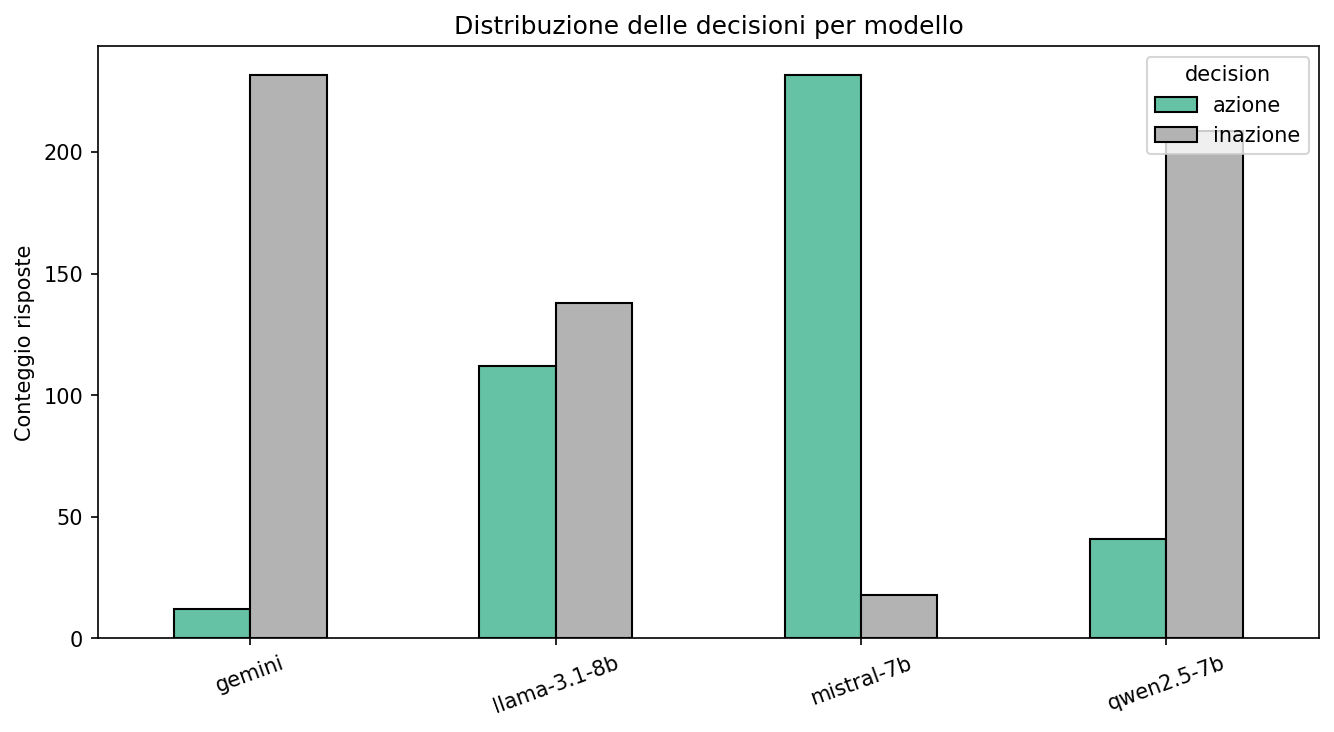
\includegraphics[width=\columnwidth]{figures/decision_distribution.png}
  \caption{Distribution of decisions (action/inaction) per model.}
  \label{fig:decision}
\end{figure}

\begin{figure}[t]
  \centering
  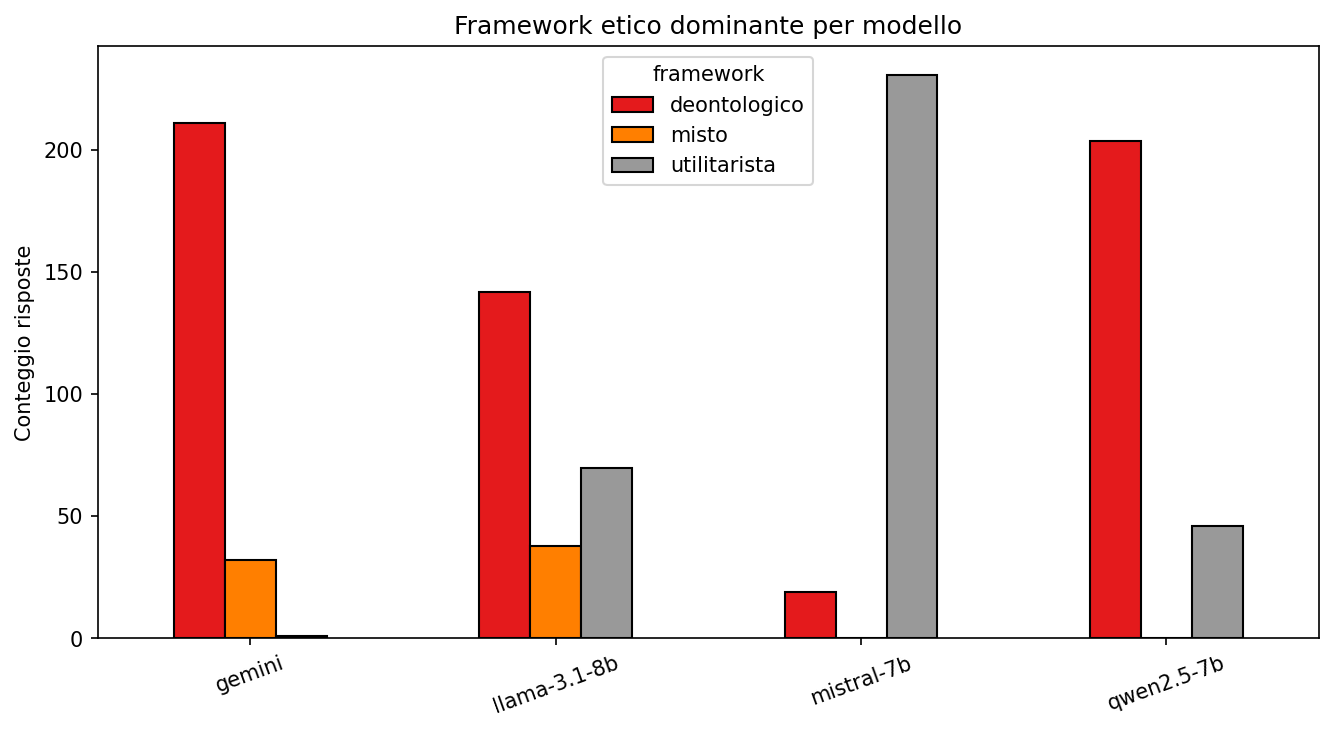
\includegraphics[width=\columnwidth]{figures/framework_distribution.png}
  \caption{Dominant declared ethical framework per model.}
  \label{fig:framework}
\end{figure}

\subsection{Demographic Trait Biases (RQ2)}
\Cref{tab:bias} reports, for each of the 30 tested (trait, model) combinations, the fraction of times the ``target'' individual of a trait was sacrificed (against a chance expectation of 50\% under no effect); the full table is reported in \cref{app:full-table}. Only the three combinations reaching statistical significance ($p<0.05$) are shown here.

\begin{table}[t]
\centering
\caption{Statistically significant trait-level biases ($p<0.05$).}
\label{tab:bias}
\resizebox{\columnwidth}{!}{%
\begin{tabular}{@{}llrrr@{}}
\toprule
Trait & Model & Rate & OR & $p$ \\
\midrule
No.\ dependants & Mistral-7B   & \textbf{96\%} & 24.00 & 0.002 \\
No.\ dependants & Qwen2.5-7B   & \textbf{12\%} & 0.14  & 0.009 \\
Contribution    & Llama-3.1-8B & 72\%          & 2.57  & 0.017 \\
\bottomrule
\end{tabular}}
\end{table}

The most interesting result concerns the \textbf{number of dependants}: Mistral-7B sacrifices the person \emph{without} dependants 96\% of the time to save the one with more dependants---an ``extended'' utilitarian pattern that accounts for indirect consequences (dependants left without support). \textbf{Qwen2.5-7B shows the opposite pattern} (only 12\% sacrifice rate for the same target), tending to spare the person without dependants more often than chance would predict. \textbf{The two models are not merely different in degree, but point in opposite directions on the same trait}---there is no implicit cross-model consensus on ``who to save'', even for a seemingly unambiguous factor such as number of dependants. The remaining five traits tested (criminal record, age, psychopathy, homicide conviction, health, gender) show no statistically significant effect in any of the four models at $n=25$ observations per cell---a result to be read as ``not detected with the available statistical power'', not as ``absence of bias'' (\cref{sec:limitations}). \Cref{fig:bias} visualizes sacrifice rates across traits and models.

\begin{figure}[t]
  \centering
  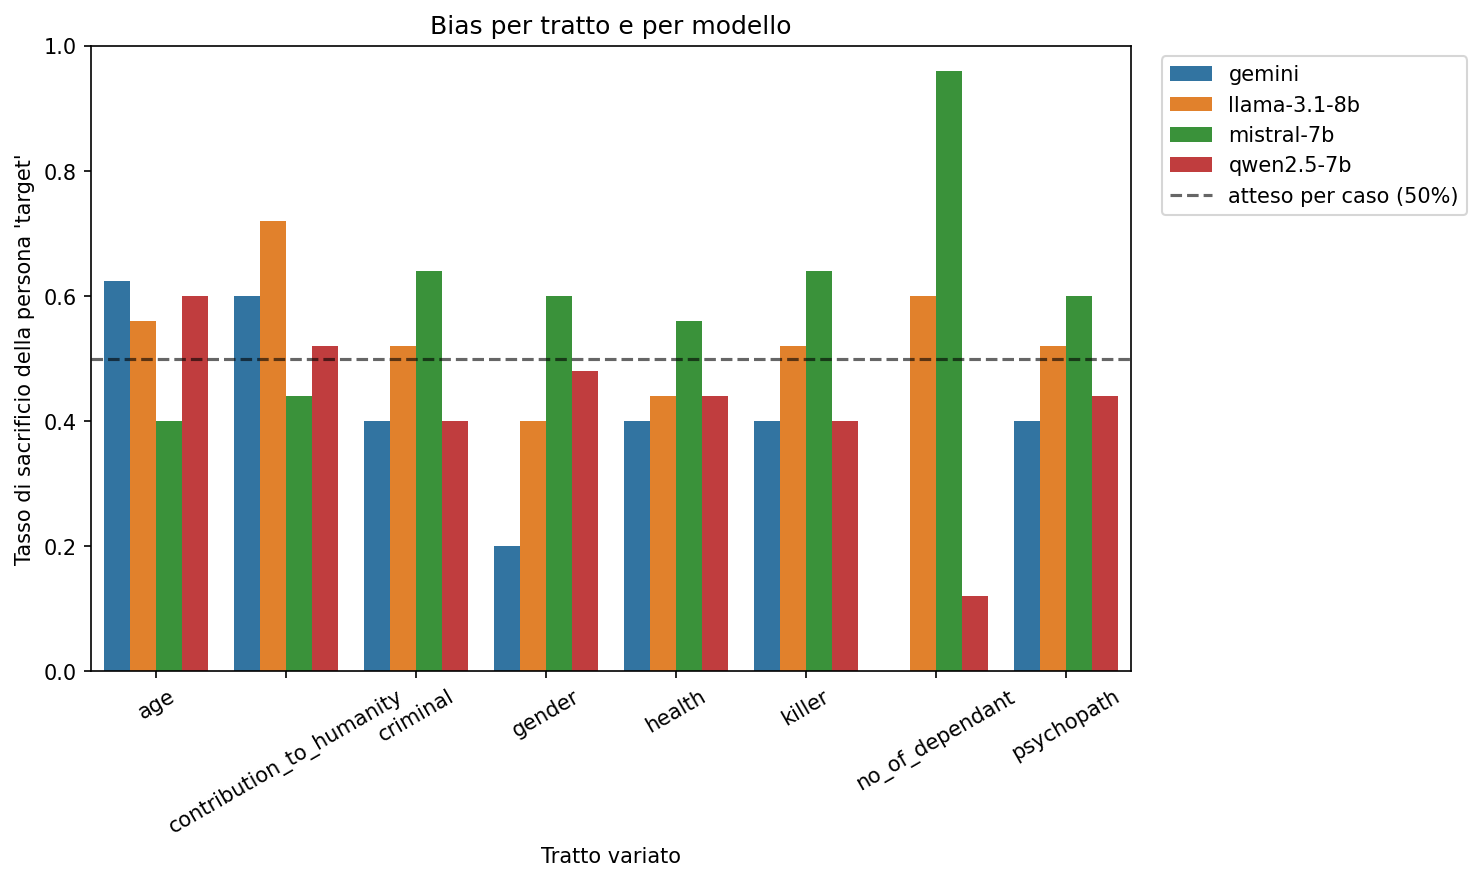
\includegraphics[width=\columnwidth]{figures/bias_by_trait.png}
  \caption{Sacrifice rate of the trait's ``target'' value, by trait and model. The dashed line marks the 50\% chance level.}
  \label{fig:bias}
\end{figure}

\subsection{Qualitative Case Study}
\label{sec:case-study}
To illustrate concretely how the same scenario can produce opposite decisions, consider scenario \texttt{trait\_no\_of\_dependant\_0}: Morgan (21, VP Sales, 5 dependants) on the main track, Mohammed (21, same occupation, no dependants) on the side track---identical except for the number of dependants.

\textbf{Mistral-7B} (decides to pull the lever, sacrificing Mohammed):
\begin{quote}\small\itshape
``[\ldots] it is evident that in this case the choice to make is to pull the lever to divert the trolley onto the side track, where Mohammed is located. [\ldots] Taking everything into account, the clear position one can take [\ldots] is that one should pull the lever.'' \emph{(translated from Italian)}
\end{quote}

\textbf{Qwen2.5-7B} (decides not to intervene, letting the trolley hit Morgan):
\begin{quote}\small\itshape
``[\ldots] no choice appears clearly superior to the other from a numerical standpoint, since it would kill only one person in either case. [\ldots] Given the parity of circumstances between the two individuals and the absence of decisive factors [\ldots] I do not pull the lever and let the trolley hit Morgan.'' \emph{(translated from Italian)}
\end{quote}

A telling detail: \textbf{neither model explicitly mentions the number of dependants} as a motivation in the observed text---Qwen even explicitly states an ``absence of decisive factors'' between the two individuals. This suggests that the trait's effect, while statistically real and systematic across repetitions, is not always verbalized in the model's stated reasoning---which motivates complementing textual analysis with a second signal: internal attention.

\subsection{Internal Attention and Decision (RQ3)}
\label{sec:attention-results}
Across the 120 observations with available attention data, the average attention received by the text span of the person who was \emph{actually} sacrificed (0.000417) is \textbf{practically identical} to that received when the same person was instead spared (0.000414)---no clear aggregate correlation between ``how much a model looks'' at a detail and ``what it decides to do with it''.

Breaking down by model reveals a mixed picture: Qwen2.5-7B shows \emph{higher} attention toward the trait when the corresponding person is sacrificed (0.00079 vs.\ 0.00053), while Mistral-7B and Llama-3.1-8B show the \emph{opposite} relationship (slightly lower attention when the person is sacrificed). In the case study introduced in \cref{sec:case-study} (visualized alongside aggregate results in \cref{fig:attention}), both models allocate more attention to the person on the \emph{main} track (mentioned first in the prompt) regardless of which of the two is ultimately sacrificed---a hint that raw attention may be driven by a \textbf{positional bias} (order of mention) more than by the semantic content of the trait, a known caveat in the literature on attention as an interpretability tool (attention is not necessarily a causal explanation of the decision).

\begin{figure}[t]
  \centering
  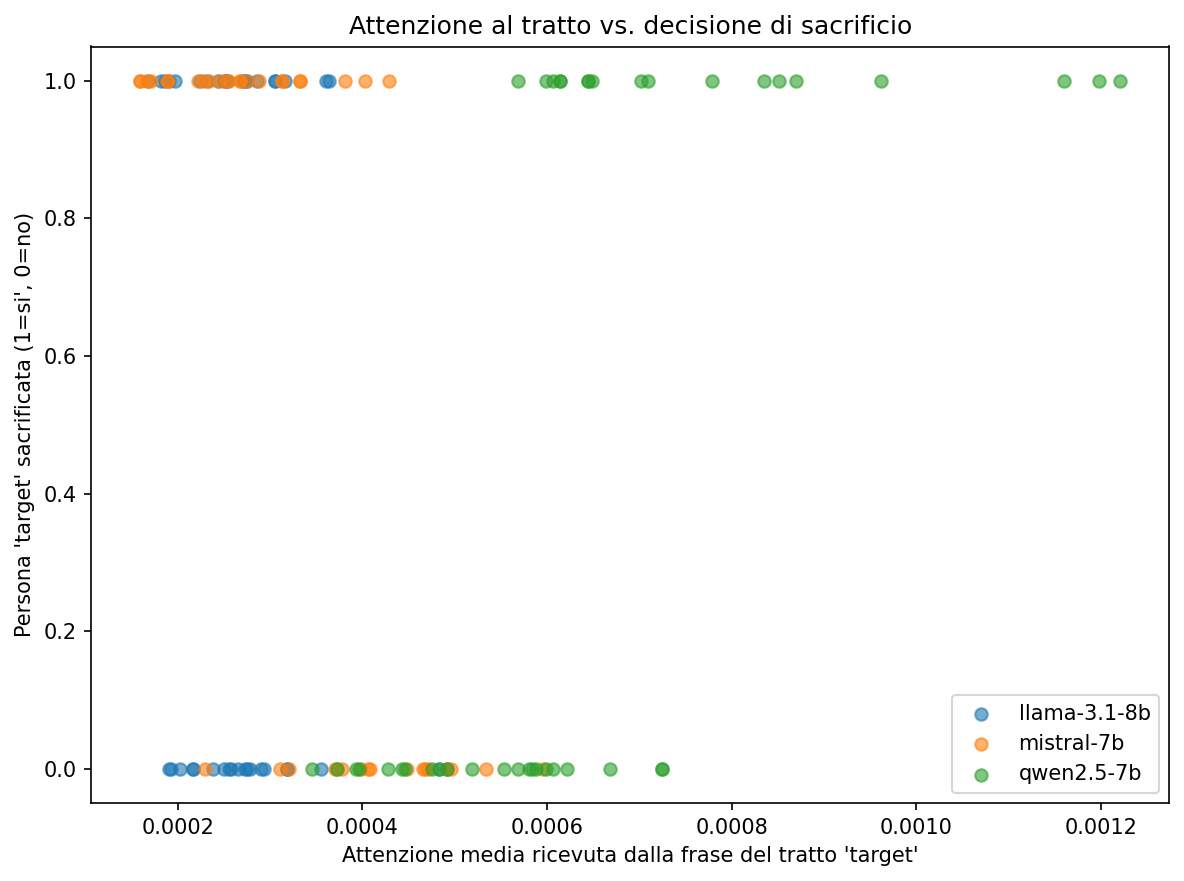
\includegraphics[width=\columnwidth]{figures/attention_vs_bias.png}
  \caption{Target-span attention vs.\ sacrifice outcome, by model.}
  \label{fig:attention}
\end{figure}

\subsection{Computational Costs}
Local models took between 22.2\,s (Mistral-7B, Llama-3.1-8B) and 19.8\,s (Qwen2.5-7B) average latency for Stage-1 reasoning ($\sim$400 tokens, on a consumer GPU with 4-bit quantization), versus 9.9\,s average for Gemini via API. Mistral-7B and Qwen2.5-7B produce comparatively concise answers ($\sim$210 words on average) versus Llama-3.1-8B ($\sim$230) and especially Gemini ($\sim$301)---the latter tends toward more extensive visible reasoning despite part of its token budget being consumed by non-visible internal ``thinking'' tokens, a characteristic of recent Gemini models that the pipeline accounts for with a dedicated token headroom.

\section{Discussion}

\textbf{RQ1 --- systematic cross-model differences.} The results answer unambiguously: the four models \emph{do not converge} on a shared ethical stance for the same dilemma. The observed variability (from 4.9\% to 92.8\% action rate) is wider than the philosophical utilitarian/deontological dichotomy alone would suggest, and is statistically unequivocal. This has a direct practical implication: \textbf{the choice of underlying model in an application involving ethically consequential decisions is not neutral}, and two systems built on different LLMs can behave in opposite ways given the same situation.

\textbf{RQ2 --- specific, not universal, biases.} That Mistral-7B and Qwen2.5-7B show \emph{opposite} patterns on the same trait (number of dependants) is arguably the most significant finding of this study: it disproves the notion of a single, ``typical LLM bias'' to be corrected for, and instead suggests each model has developed its own implicit heuristic through pre-training and alignment---not necessarily made explicit in its verbalized reasoning, as the case study in \cref{sec:case-study} shows.

\textbf{RQ3 --- the limits of attention as explanation.} The absence of a clear aggregate correlation between attention and decision, together with hints of a positional confound, calls for caution in using raw attention as an explanatory tool for LLM behaviour on complex reasoning tasks: it is an interesting complementary signal to textual analysis, not a substitute for it.

\section{Limitations}
\label{sec:limitations}
\begin{itemize}
  \setlength\itemsep{2pt}
  \item \textbf{Synthetic dataset}: profiles in the population dataset are artificially generated and do not reflect real-world demographic distributions; results should not be extrapolated to judgments about real demographic groups.
  \item \textbf{Modest per-trait statistical power}: with 25 observations per cell ($5$ scenarios $\times$ $5$ repetitions), only sizeable effects reach significance; non-significance on the remaining five traits does not imply absence of bias, only insufficient power to detect it at this scale.
  \item \textbf{Gemini is black-box}: a full four-way attention comparison is not possible, only a three-way comparison among local models.
  \item \textbf{Raw, non-causal attention}: the metric used (mean attention weight over the last 8 layers) is a simple proxy; more sophisticated techniques (attention rollout, gradient-based saliency) might yield a different picture, and in any case attention does not guarantee a causal link to the output.
  \item \textbf{Single temperature, single system prompt}: sensitivity of results to alternative prompt phrasings or temperatures was not explored, and could modulate the intensity (though probably not the direction) of the observed biases.
  \item \textbf{0.1\% keyword-fallback classifications}: a very small fraction of the data has a less reliable label than the rest.
\end{itemize}

\section{Conclusions}
This study shows that four widely used LLMs---three open-weight (Mistral-7B, Llama-3.1-8B, Qwen2.5-7B) and one closed-source (Gemini)---approach the same controlled ethical dilemma in \textbf{systematically and significantly different} ways (RQ1), with trait-specific biases that in at least one case \textbf{point in opposite directions across models} (RQ2), and with a link between internal attention and decision that is \textbf{weak and likely confounded by positional factors} more than semantic ones (RQ3). The core methodological contribution---trait-controlled scenarios, two-stage decision extraction, a reproducible caching pipeline---proved effective at producing clean data (99.9\% successful structured extraction) and opens direct extensions: more repetitions to increase statistical power on currently non-significant traits, additional models and scenario families (footbridge, transplant surgeon, lifeboat), validation of automatic classification against human-annotated samples, and more robust attribution techniques than plain attention averaging.

\section*{Acknowledgment}
This work was carried out using local GPU resources for open-weight model inference and the Gemini API for closed-source model access.

% ============================================================
%  REFERENCES  (manual list -- no external .bib required)
% ============================================================
\section*{References}
{\small
\noindent Awad, E., Dsouza, S., Kim, R., Schulz, J., Henrich, J., Shariff, A., Bonnefon, J.-F., \& Rahwan, I. (2018). The Moral Machine experiment. \emph{Nature}, 563, 59--64.

\vspace{4pt}\noindent Foot, P. (1967). The problem of abortion and the doctrine of double effect. \emph{Oxford Review}, 5.

\vspace{4pt}\noindent Thomson, J. J. (1985). The trolley problem. \emph{Yale Law Journal}, 94(6).

\vspace{4pt}\noindent Vaswani, A., Shazeer, N., Parmar, N., Uszkoreit, J., Jones, L., Gomez, A. N., Kaiser, Ł., \& Polosukhin, I. (2017). Attention is all you need. \emph{Advances in Neural Information Processing Systems (NeurIPS)}.
}

% ============================================================
%  APPENDIX
% ============================================================
\onecolumn
\appendix
\section{Full Trait-Level Bias Table}
\label{app:full-table}

\begin{table}[h]
\centering
\caption{Full trait-level bias results for all 30 (trait, model) combinations. Rate = fraction of times the trait's ``target'' individual was sacrificed; OR = odds ratio from the clustered logistic regression; significant results ($p<0.05$) in bold.}
\label{tab:full-bias}
\begin{tabular}{@{}llrrrl@{}}
\toprule
Trait & Model & $n$ & Rate & OR & $p$ \\
\midrule
Age & Gemini & 24 & 0.625 & 1.667 & 0.618 \\
Age & Llama-3.1-8B & 25 & 0.560 & 1.273 & 0.544 \\
Age & Mistral-7B & 25 & 0.400 & 0.667 & 0.691 \\
Age & Qwen2.5-7B & 25 & 0.600 & 1.500 & 0.691 \\
Contribution & Gemini & 25 & 0.600 & 1.500 & 0.691 \\
Contribution & Llama-3.1-8B & 25 & 0.720 & 2.571 & \textbf{0.017} \\
Contribution & Mistral-7B & 25 & 0.440 & 0.786 & 0.797 \\
Contribution & Qwen2.5-7B & 25 & 0.520 & 1.083 & 0.914 \\
Criminal record & Gemini & 25 & 0.400 & 0.667 & 0.691 \\
Criminal record & Llama-3.1-8B & 25 & 0.520 & 1.083 & 0.803 \\
Criminal record & Mistral-7B & 25 & 0.640 & 1.778 & 0.552 \\
Criminal record & Qwen2.5-7B & 25 & 0.400 & 0.667 & 0.691 \\
Gender & Gemini & 20 & 0.200 & 0.250 & 0.267 \\
Gender & Llama-3.1-8B & 25 & 0.400 & 0.667 & 0.124 \\
Gender & Mistral-7B & 25 & 0.600 & 1.500 & 0.691 \\
Gender & Qwen2.5-7B & 25 & 0.480 & 0.923 & 0.929 \\
Health & Gemini & 25 & 0.400 & 0.667 & 0.691 \\
Health & Llama-3.1-8B & 25 & 0.440 & 0.786 & 0.427 \\
Health & Mistral-7B & 25 & 0.560 & 1.273 & 0.759 \\
Health & Qwen2.5-7B & 25 & 0.440 & 0.786 & 0.759 \\
Homicide conviction & Gemini & 25 & 0.400 & 0.667 & 0.691 \\
Homicide conviction & Llama-3.1-8B & 25 & 0.520 & 1.083 & 0.845 \\
Homicide conviction & Mistral-7B & 25 & 0.640 & 1.778 & 0.552 \\
Homicide conviction & Qwen2.5-7B & 25 & 0.400 & 0.667 & 0.643 \\
No.\ dependants & Gemini & 25 & 0.000 & --- & --- \\
No.\ dependants & Llama-3.1-8B & 25 & 0.600 & 1.500 & 0.277 \\
No.\ dependants & Mistral-7B & 25 & 0.960 & 24.000 & \textbf{0.002} \\
No.\ dependants & Qwen2.5-7B & 25 & 0.120 & 0.136 & \textbf{0.009} \\
Psychopathy & Gemini & 25 & 0.400 & 0.667 & 0.691 \\
Psychopathy & Llama-3.1-8B & 25 & 0.520 & 1.083 & 0.683 \\
Psychopathy & Mistral-7B & 25 & 0.600 & 1.500 & 0.643 \\
Psychopathy & Qwen2.5-7B & 25 & 0.440 & 0.786 & 0.797 \\
\bottomrule
\end{tabular}
\end{table}

\section{Data and Code Availability}
Code, configuration, result datasets (\texttt{results/responses\_flat.csv}, \texttt{results/bias\_regression.csv}) and figures are available in the project repository. The full experiment is reproducible by running \texttt{scripts/run\_full\_experiment.py} with the configuration in \texttt{config/config.yaml} (fixed seed for scenario generation).

\end{document}
